\documentclass[12pt,a4paper]{article}
\usepackage[utf8]{inputenc}
\usepackage{array}
\usepackage{booktabs}
\usepackage{graphicx}
\usepackage[usenames,dvipsnames]{color}
\usepackage{dirtytalk}
\usepackage[margin=0.5in]{geometry}

\usepackage[maxnames=5]{biblatex}
\addbibresource{refs.bib}

\usepackage{hyperref}
\hypersetup{
  colorlinks,
  citecolor=blue,
  filecolor=black,
  linkcolor=[rgb]{0.1,0.3,0.7},
  urlcolor=black
}

\setlength{\parindent}{0pt}
\frenchspacing

\addtolength{\oddsidemargin}{0.2in}
\addtolength{\evensidemargin}{0in}
\addtolength{\textwidth}{-0.5in}
\addtolength{\topmargin}{-0.05in}

\begin{document}
  \begin{center}
    
\includegraphics[width=90mm]{logo.png}\\
    \vspace{3mm}

    \vspace{3mm}
    \Huge{\textbf{REGIUS MARK}}\\
    \vspace{3mm}
    \normalsize{www.regiusmark.io}\\
    \normalsize{contact@regiusmark.io}\\
    \normalsize{December 7, 2020}

    \vspace{30mm}
    \Large{\textbf{White Paper}}\\
    \large{Proposed Ticker symbol: MARK}\\
    \vspace{30mm}

    \large{\textbf{Our mission is to bring utility to precious metals in}}\\
    \large{\textbf{an innovative blockchain solution --- Enter the Golden Age.}}

    \vspace*{\fill}
    \normalsize{Copyright ©2020 The RegiusMark Group Ltd. All Rights Reserved.}
  \end{center}

  \newpage
  \begin{center}
    \large{\textbf{DISCLAIMER OF LIABILITY}}
  \end{center}

  \begin{center}
    \textbf{\underline{Legal Disclaimer}}
  \end{center}

  DISCLAIMER PLEASE READ THIS DISCLAIMER SECTION CAREFULLY. IF YOU ARE IN ANY
  DOUBT AS TO THE ACTION YOU SHOULD TAKE, YOU SHOULD CONSULT YOUR LEGAL,
  FINANCIAL, TAX, OR OTHER PROFESSIONAL ADVISOR(S).\\ % chktex 36

  Please read the following notice carefully before proceeding to read this
  Whitepaper document issued by \textbf{THE REGIUSMARK GROUP LTD}, an exempted
  company incorporated and existing under the laws of the Cyprus with registered
  office in headquartered in Cyprus.\\

  \textbf{THE REGIUSMARK GROUP LTD}.reserves the legal right to post changes to
  the Whitepaper at any time, and by continuing reading the Whitepaper
  thereafter, you agree to be bound by the latest version of the Whitepaper. If
  any changes on the Whitepaper are not acceptable, you must not contribute to
  in exchange for the \textbf{Token}. In this Legal Disclaimer, \textbf{``Regius
  Token''} or \textbf{``Regius Mark Tokens'' ``Regius Mark'' ``Regius''
  ``Mark''} or \textbf{``Token''} and \textbf{``We''} refers to \textbf{THE
  REGIUSMARK GROUP LTD}, and \textbf{``User''} or
  \textbf{``you''} refers to each reader of the Whitepaper and contributor in
  exchange for the Token.\\

  \textbf{This notice applies to all persons who read this document. Please note
  this notice may be altered or updated.}\\

  The information set forth below may not be exhaustive and does not imply any
  elements of a contractual relationship while we make every effort to ensure
  that any material in this Whitepaper is accurate and up to date, such material
  in no way constitutes the provision of professional advice.\\

  This Whitepaper does not constitute a prospectus or offer document of any sort
  and is not intended to constitute an offer of securities or a solicitation for
  investments in securities in any jurisdiction.\\

  This Whitepaper is for information purposes only. The contents of this
  Whitepaper are not a financial promotion. Therefore, none of the contents of
  this Whitepaper serves as an invitation or inducement to engage in any sort of
  investment activity.\\

  The contents and details provided within this current English Whitepaper,
  supersede and replace all other previous whitepaper editions as well as all
  other whitepaper translations in existence.\\

  This whitepaper does not constitute an official agreement of any kind and the
  information provided herein is for informational purposes only. Project
  parameters, dates, specifications provided as well as other details technical
  or not are subject to change without prior notice.\\

  By participating in the Token Distribution, you must agree to the Regius Mark
  Terms \& Conditions (Terms of Use). The Token does not have the legal
  qualification of a security, since it does not give any rights on dividend or
  interest. The Token is final and non-refundable. The Token is not a share and
  does not give any right to participate to the general meeting of the Company.
  The Token cannot have a performance or a value outside the platform or another
  affiliate platform/application. The purchase and use of the Token shall
  therefore not be done for speculative usage.\\

  Acquisition of Tokens does not present an exchange of cryptocurrencies for any
  form of ordinary shares of the Distributor and a Holder of Tokens is not
  entitled to any guaranteed form of dividend and/or any other rights what’s so
  ever.

  \begin{center}
    \textbf{\underline{Risk Statements}}
  \end{center}

  Prospective acquirers of the Tokens should carefully consider and evaluate all
  risks and uncertainties associated with the cryptocurrencies, and their
  respective businesses and operations and the Tokens. Familiarize yourself with
  all the information set out in this Whitepaper, Risk Notice prior to any
  contribution in exchange of the Tokens.\\

  Tokens neither guarantees nor accepts responsibility for the accuracy,
  reliability, current (as of this White Paper) or completeness of this content.
  Individuals intending to contribute in the blockchain platform should seek
  independent professional advice prior to acting on any of the information
  contained in this paper.\\

  Any person undertaking to acquire Tokens must be aware that the Regius Mark
  business model may change or need to be modified because of new regulatory and
  compliance requirements from any applicable laws in any jurisdictions. In such
  case, any person undertaking to acquire Tokens, acknowledge and understand
  that neither Regius Mark nor any of its affiliates shall be held liable for
  any direct or indirect loss or damages caused by such changes and that project
  parameters, dates, specifications provided as well as other details technical
  or not could be subject to change without prior notice.\\

  In addition, Regius Mark has the complete freedom to operate or domicile its
  business(s) anywhere suitable provided it complies with the regulatory
  framework of the requisite jurisdiction.\\

  The Tokens are not securities and participants comprehend and fully accept the
  fact that Tokens are not securities under any circumstance, neither are they
  registered with any government entity as a security.\\

  No regulatory authority has examined or approved any of the information set
  out in this Whitepaper. No such action has been or will be taken under the
  laws, regulatory requirements or rules of any jurisdiction. The publication,
  distribution or dissemination of this Whitepaper does not imply that the
  applicable laws, regulatory requirements, or rules have been complied.\\

  Ethereum related risks to tokens will be issued on the Ethereum blockchain
  thus being dependent on it. The functionality of the Regius Mark Tokens will
  be severely affected should the Ethereum protocol malfunction or fail.\\

  Risks associated with quantum computers despite the efforts made by the
  blockchain community to safeguard the security of cryptocurrency technology,
  the potential development and deployment of quantum computers or any other
  kind of advanced types of computers in the future may put this security at
  risk. In such a case, the Token will be affected as well.\\

  No fund insurance provided. Any and all types of funds collected in any period
  are in no way insured. Funds may lose their value in whole or completely
  without warning. There is no insurance company, private or public, to turn to
  should something goes wrong with the funds provided.

  \begin{center}
    \textbf{\underline{Restricted Areas}}
  \end{center}

  Acquiring and storing the Tokens involves various risks, that Regius Mark with
  its affiliates may not be able to launch its operations and develop its
  platform. Therefore, and prior to acquiring the Token, you should carefully
  consider the risks, costs, and benefits of acquiring the The Regius Mark Token
  within the Crowd Sale, Citizens, residents (tax or otherwise) and green card
  holders of the United States of America, Singapore, China or other U.S. or
  Singapore Person are exempt from buying the Tokens. The term “U.S. or
  Singapore Person” or ‘’Chinese Person’’ or ‘’German Person’’ refers to anyone
  who lives in the United States or Singapore or China or Germany or any entity
  that is incorporated under United States or Singapore law or Chinese Law or
  Germany Law. American citizens living abroad, Chinese Persons living abroad,
  Singaporeans living abroad and Germans living abroad, can also be considered
  “domiciled” Under certain conditions.\\

  After reading the Whitepaper you may decide to take part in the development of
  new Decentralized Security, using your knowledge, time and financial resources
  prior contributing. Therefore, by reading this text, you assume the
  unconditional obligation that, in the event of being a citizen of USA, China,
  Singapore or any other country, any lawsuit with any claimant, where your name
  is featured as an involved party, we receive a guaranteed right to charge you
  as a private party for the full amount of losses, including any fines or legal
  costs, including in the event of your using software (VPN, Class Action, etc)
  to conceal your true country of residence.\\

  This Whitepaper, or any part thereof, as well as any copies, must not be taken
  or transmitted to any country where distribution or dissemination of this
  Whitepaper is prohibited or restricted. The Token distribution and further
  existence is subject to and governed by Cyprus Law to the exclusion of Cyprus
  Law and any International Treaties. You and the Regius Mark agree to seek an
  amicable settlement prior to bringing any legal action. All disputes arising
  from or under the white paper are ruled by the Terms \& Conditions accepted by
  you during the crowd sale and shall be resolved by arbitration in accordance
  with the Cyprus Rules of International Arbitration of the Cyprus Chambers of
  Commerce in force on the date when the Notice of Arbitration is submitted in
  accordance with these Rules. The arbitration panel shall consist of one
  arbitrator only. The seat of the arbitration shall be in the Republic of
  Cyprus unless otherwise informed by Regius Mark prior the start of it. The
  arbitral proceedings shall be conducted in English.

  \newpage
  \tableofcontents
  \newpage

  \section{Introduction}
  Cryptocurrencies such as Bitcoin have been successful examples in creating a
  distributed network that users could trust, and many of these currencies have
  experienced a tremendous increase in value, regardless of having no backing.
  It has marked a significant beginning to the digital currency world that users
  can trust, becoming what many have called ``digital gold''.\\

  Currency markets are volatile where our token, MARK, will be backed by
  physical gold providing stability and minimizing risk. The blockchain provides
  a means to secure funds digitally without weighing you down. Our technology is
  designed to be eco-friendly and easy to use for the average consumer.\\

  Decentralized networks have good intentions but we see it leads to issues such
  as scalability, performance, and inability to upgrade the software easily. Our
  centralized network allows us to scale, optimize for performance, and easily
  upgrade the system.\\

  The Regius Mark blockchain will contain one virtual asset with the name of
  MARK. These virtual assets will be backed by physical gold,
  ensuring a stable market, rather than a volatile market.

  \section{Current Issues}
  There are a variety of issues in the financial system and existing
  cryptocurrencies that prevent wide-scale adoption by the user and
  merchants. There are risks involved for the merchant and the consumer.\\

  The common risk is a consequence of the volatile nature of the cryptocurrency
  markets. This volatility is notably caused by tokens that have no intrinsic
  value, relying on the trust and faith of its users to bring value. The
  volatility helped drive new technologies that are increasingly sophisticated
  for the merchants and users alike. However, both have to account for the
  ever-changing landscape of the token values. By physically stabilizing our
  token to gold, we get the benefits of the gold standard.\\

  When blockchains are under heavy load, the fees become expensive. The
  underlying technology is not designed to scale. Modern advances and research
  into algorithms allow us to create new technologies designed to be scalable
  for the world.\\

  The technology is still too difficult to use for the consumer and business
  owner alike. There's a problem when merchants have to use third-party payment
  processors to accept payments on the blockchain and users have to decide which
  wallet to use and learn how it works. We aim to have an intuitive wallet with
  native multi-signature support for consumers and SDKs designed to interact
  with the blockchain made available for merchants. The current lack of DX and
  UX is a hindrance to global adoption.\\

  Consumers want the cheapest fees when making transactions. Tech-savvy crypto
  users will hold a wide portfolio of tokens and decide which blockchain is the
  most cost effective to create a transaction. A novice will be forced to
  struggle with the expensive fees and time-to-time even the tech-savvy will
  have to as well.\\

  \newpage
  The Proof-of-Work algorithm is a dinosaur in the modern era of computer
  science. A Bitcoin specialist has determined it takes over an estimated 2.5
  gigawatts of electricity to mine. We are phasing out these expensive
  algorithms and replacing them with an eco-friendly system that is designed to
  scale and confirm transactions quickly. The efficiency is essential to enable
  a positive experience for the merchant and consumer.\\

  \section{Utility Purpose}
  The tokens issued are derived by the proof of gold assets stored within the
  platform, providing the stability a cryptocurrency needs to be useful for any
  user and business. Holders of the token are provided the right to a product or
  service at the discretion of an entity accepting the token.

  \section{Use of Funds}
  The majority of contributions raised through tokenization activities will be
  used to acquire gold. Some funds will be used for further research and
  development on our digital infrastructure. We will continue to make
  improvements on our blockchain, expand distribution mechanisms, acquire
  exchange listings, and satisfy associated operating costs and overhead
  expenses.

  \vspace{5mm}
  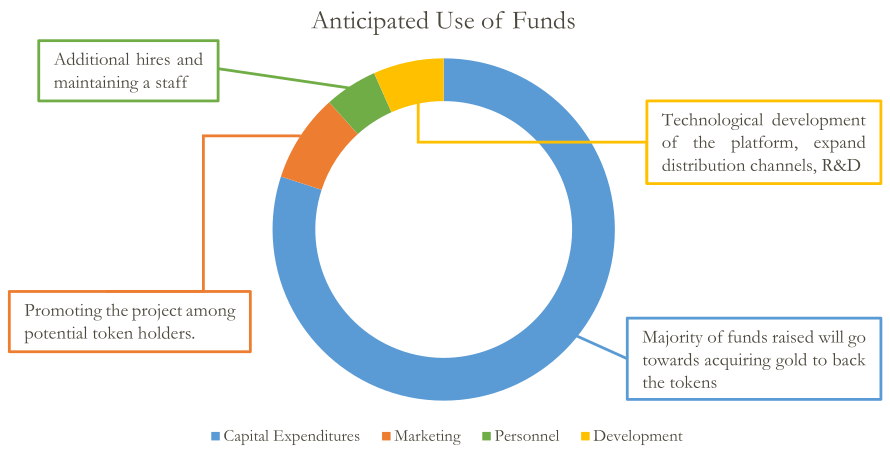
\includegraphics[width=\linewidth]{anticipated-use-of-funds.png}

  \section{Technology}
  We have seen blockchains provide a secure tamper-resistant database.
  Operations performed are deterministic allowing for the history to be
  verified. Any client will be able to synchronize the blockchain to validate
  past transactions as well as confirm the validity of future transactions.\\

  \subsection{Centralized}
  Being backed by physical assets requires a strong authority to strive
  properly. These assets may be handled by third-party brokers which present a
  proof of ownership to the network authorities. The authority will have
  permission to mint new tokens and store the associated documents including
  the distribution of these tokens.

  \subsection{Smart Contract VM}
  The virtual machine is used to execute smart contract bytecode. In Regius
  Mark, a stack machine is used with a forth-like scripting language. The
  bytecode supports a minimal set of opcodes required for financial services
  without adding unnecessary functionality to accomplish our goal. The opcodes
  used must be deterministic based on the current state of the blockchain.

  \subsection{Wallet}
  Wallets have been increasingly becoming easier to use by the user for
  basic transactions. However, these interfaces are too simple for the power
  user. Our interface will be versatile to the varying scenarios from simple
  tasks to the complex. Performing complex tasks by the power user should be as
  straight forward as the novice sending a transaction.\\

  The wallet experience and interface must be simple and intuitive for all
  users. Multi-signature wallets will be supported out of the box. A friend
  system can be used to create new wallets and sign a multi-signature
  transaction with the click of a few buttons. This system can also be used by
  merchants to accept payments and allow users to track who owns the address
  they sent the funds.\\

  For our expert users, advanced options and script builders will be available.
  The UI will be simple yet feature rich to avoid hindering expert users and
  ease new users getting into advanced smart contracts.

  \subsection{Security}
  Blockchains inherently need to be a fortress. All transactions are signed to
  prove the authenticity of the owner to perform an action on the blockchain.
  Regius Mark will support multi-signature wallets and smart contracts where
  higher levels of security are necessary.\\

  \newpage
  The centralized nature does not diminish the security of our infrastructure.
  The blockchain can be synchronized across the world in real time providing
  durability and tamper resistance as blockchain history cannot be rewritten.
  The master node will be using a multi-signature cold storage wallet and
  separate keys only for block production.

  \subsection{Transparency}
  Blockchains are naturally sequential and contain all the necessary data that
  pertains to the system. This allows us to easily distribute the block log
  without worrying about additional metadata. Any node operators will be able to
  synchronize the log and be able to remain in sync as new blocks arrive.

  \subsection{Minting}
  Blocks will be produced through a process called minting every three seconds.
  This process can only occur by use of a master node. The Regius Mark team will
  be the only master node on the network.\\

  Unlike traditional cryptocurrencies with block rewards, Regius Mark does not
  partake in the creation of tokens unless explicitly created by a master node
  during minting a new block. This is a necessary step to ensure that we never
  overcommit circulating tokens, in this way we never exceed our physical asset
  reserves.\\

  Minting transactions will contain data pertaining to any document providing
  proof of ownership of physical gold.

  \subsection{Fees}
  Transaction fee costs start with a minimum fee. For every additional
  transaction accepted within the block window, the minimum fee is exponentially
  multiplied by the number of transactions accepted from the applicable address.
  The fee costs will reset back to the minimum fee after the block window is
  reset. The block window is reset when transactions are halted on the address
  for a period of time.\\

  In addition to the address fee mentioned in the above paragraph, there is an
  associated \say{global} network fee. The network fee works in the same way as
  the address based fee and protects the network from flooding via multiple
  addresses. The global fee is dynamically adjusted based on network usage.\\

  This quickly gets expensive for an attacker attempting to Denial-of-Service
  (DoS) the network, but allows flexibility for a normal user when waiting for
  the block window to reset back to the minimum fee is not an option.\\

  Our fees will remain low because of our dynamic fee model allowing us to
  adjust costs based on network usage. Any fees collected will be rewarded to
  the network operators.\\

  \newpage
  Sample based on transferring funds with a minimum fee of 0.0050 coins with a
  1.5000 multiplier:

  \vspace{3mm}
  \begin{tabular}{@{}lr@{}}
    Fees & Block Height     \\ \toprule
    0.0050 & 10             \\
    0.0075 & 11             \\
    0.0112 & 12             \\
    0.0050 & $\leftarrow{}$ block window reset $\rightarrow{}$ 20 \\ \midrule{}
    Total Fees & 0.0287     \\
    \bottomrule
  \end{tabular}

  \subsection{Message Signing}
  A signature is used to confirm the authenticity of the owner or owners of a
  particular message or document. Blocks produced by the minter and transactions
  created by the user are signed using the \textit{Ed25519}\cite{ed25519}
  algorithm.\\

  Ed25519 is a modern signing algorithm, it provides a similar protection level
  to NIST P-256 and has fast verification times with small signatures. This
  particular algorithm is capable of even faster batch verification using the
  Pippenger's method or the Bos-Coster method for scalar multiplication as
  mentioned in the Ed25519 paper.\\

  Ed25519 has fewer attack vectors, such as resistance to side-channel attacks
  and attacks from poor random number generator implementations. While
  non-deterministic algorithms can suffer from hardware fault attacks, it is
  extremely difficult to successfully execute. Even with a server running
  without ECC memory the attack isn't practical in any way over the
  internet.

  \subsection{Scaling}
  Scalability can be achieved through vertical or horizontal machine deployment.
  Vertically scaling the hardware is easy to maintain, but the costs may become
  infeasible as hardware requirements increase to process the influx of
  transactions being added to the network. We will use horizontal deployment
  through different types of nodes that serve a specific function to spread the
  workload across multiple machines.\\

  The majority of processing power required will be for transaction validation.
  We will use validator nodes to validate transactions being broadcasted to the
  network. The master node relies on the correctness of the validator to ensure
  that bad transactions cannot be added to the blockchain state.\\

  \subsubsection{Security}
  Each validator will contain an Ed25519 key utilized as an identity. The master
  node will send a challenge that the validator must sign to prove the machine
  is trusted. The link between the nodes must use the latest version of TLS to
  prevent any man in the middle or replay attacks.

  \newpage
  \section*{External Links}
  \begin{itemize}
    \item{\url{https://regiusmark.io}}
    \item{\url{https://github.com/RegiusMark}}
  \end{itemize}
  \printbibliography{}
\end{document}
